% !tex root = ../Thesis.tex

This literature review attempts to cover all the subjects relevant to pitch
correction. Music theory is investigated first, covering the topics of human pitch
perception and tuning. This section attempts to determine what it means for a
pitch to be correct and how this relates to frequency. The idea is to get a list
of correct frequencies derived from a tuning system. After it is well-known what
is musically considered to be a correct pitch, the general structure of how pitch
correction is approached is investigated. This structure naturally splits up into
modules and each module is investigated further.

\section{Music Theory}

The intent of this section is to come up with a definition of what will be a
considered correct pitch. Some foundational work is required to define basic
musical concepts in a rigorous way. To start we need to define exactly what is
meant by a musical note.

A note is a sound made from a musical instrument. It has a pitch, volume, timbre
and length. These are the characteristics a musician would consider when composing
a piece of music. Each of these characteristics have a more rigorous scientific
counterpart they are related to. Pitch relates to frequency; Volume relates to
amplitude; timbre relates to harmonic content and length relates to duration. The
characteristic pair relevant to pitch correction is the pitch and frequency pair
and needs to be covered in more depth.

\begin{wrapfigure}{L}{0.5\textwidth}
\includegraphics[width=0.5\textwidth,trim={1mm 0mm 20mm 8mm},clip]{Frequency-Vs-Pitch}
\caption{"Frequency vs Pitch"}
\label{fig:FrequencyVsPitch}
\end{wrapfigure}

Pitch and frequency are terms often used interchangeably but does not refer to the
same concept. Pitch is a \textit{sensation} experienced by humans when they hear
notes containing frequencies between 31 Hz and 17.6 kHz\cite{Hearing}. The
sensation of pitch is scaled on a subjective ``high'' and ``low'' scale. The
higher the frequency, the higher the pitch perceived and the lower the frequency,
the lower the pitch perceived. This relationship between pitch and frequency is
generally considered to be logarithmic. Slight deviations from the expected
logarithmic relationship was found\cite{PitchVsFrequency} but was deemed minor
and unnecessary to incorporate for this project.

In Figure \ref{fig:FrequencyVsPitch} the relationship of frequency and pitch is
shown. Pitch is generally denoted by letters ranging from A to G with
sharps(\musSharp) and flats(\musFlat) called accidentals.  This is due to a long
history of convention and is irrelevant for now. The main takeaway is that the
perceived change in pitch is constant for each successive note. From this graph it
can be seen that frequency is exponentially dependent on pitch, or inversely,
pitch is logarithmically dependent on frequency.

From Figure \ref{fig:FrequencyVsPitch} a list of correct frequencies is obtained.
The method by which this list is obtained, originates from a concept called pitch
harmony. Two notes sounds good or in tune if their frequencies produce a simple
ratio\cite{Harmony}. For example an octave produces a ratio of 1:2 and a perfect
5th produces a ratio of 3:2. Figure \ref{fig:Harmony} shows how these two
harmonies are seen when their waveforms are plotted. The superposition created by
the two notes creating the interval has a short repeating pattern. The fact that
this pattern is short corresponds to the property of a simple ratio of
frequencies.  This short pattern/simple ratio is the origin of why two notes sound
harmonious.

\begin{figure}[h]
\centering
{\bf Octave Interval}
\begin{tabular}{c c c}
	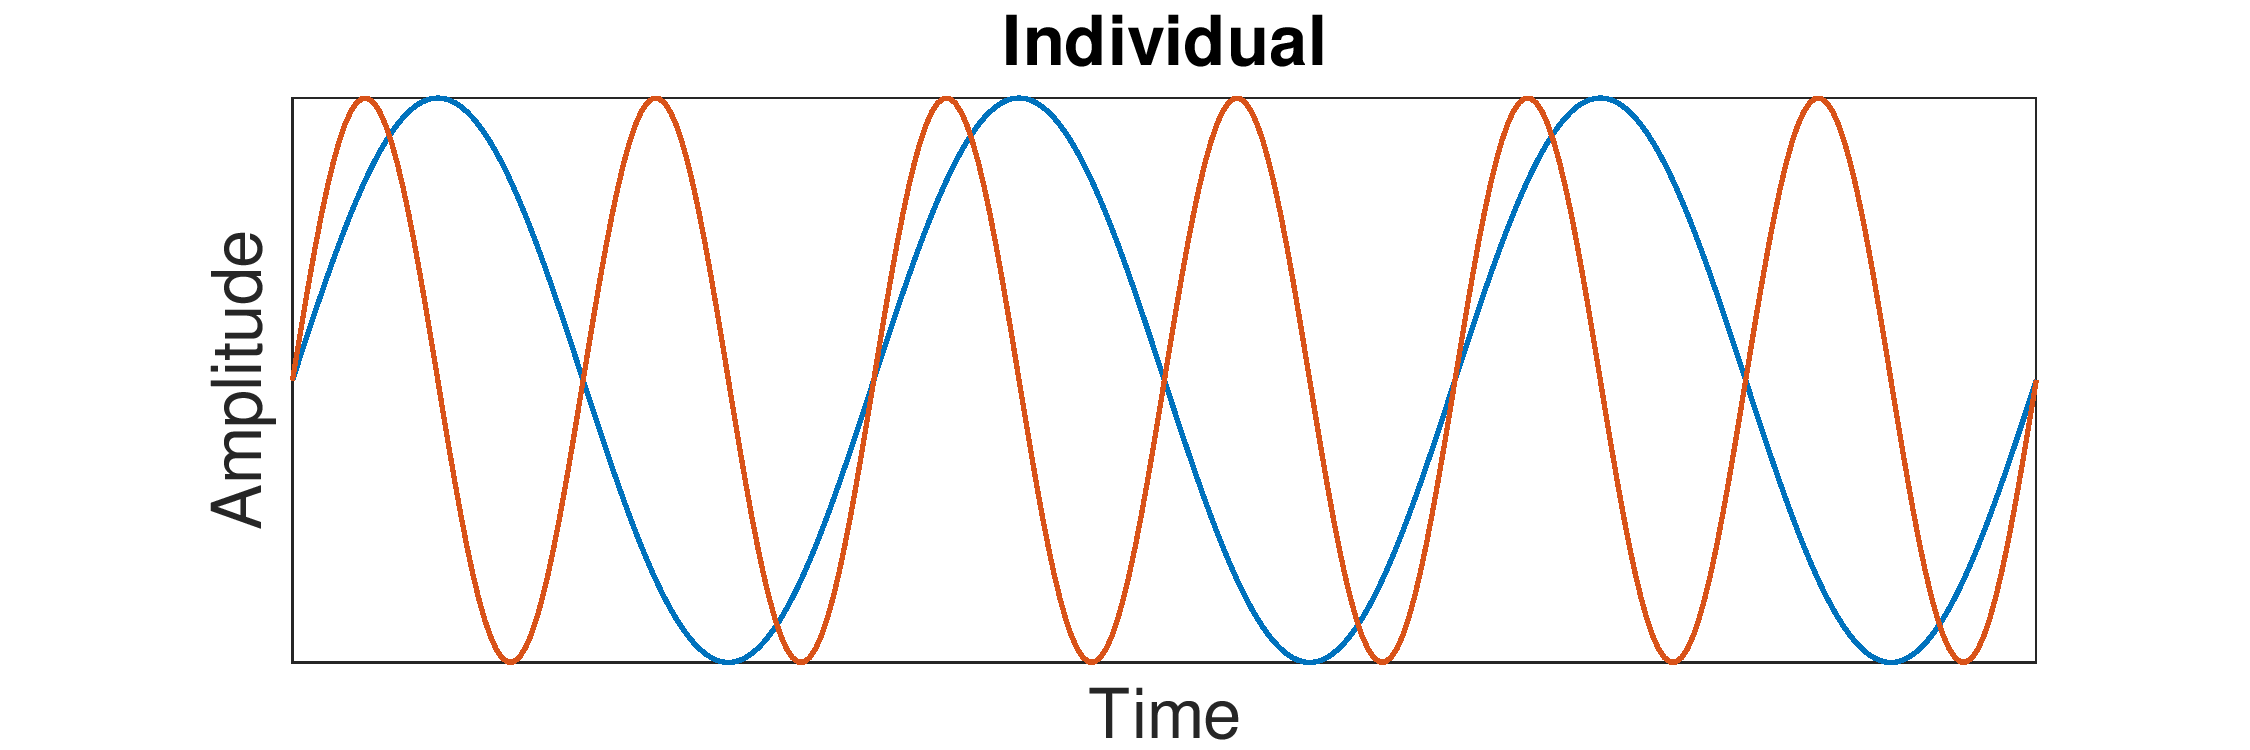
\includegraphics[align=c, width=0.4\textwidth,
		trim={3.5cm 0 3.5cm 0},clip]
		{HarmonyOctaveSeparate}

	& \huge$\rightarrow$ &
	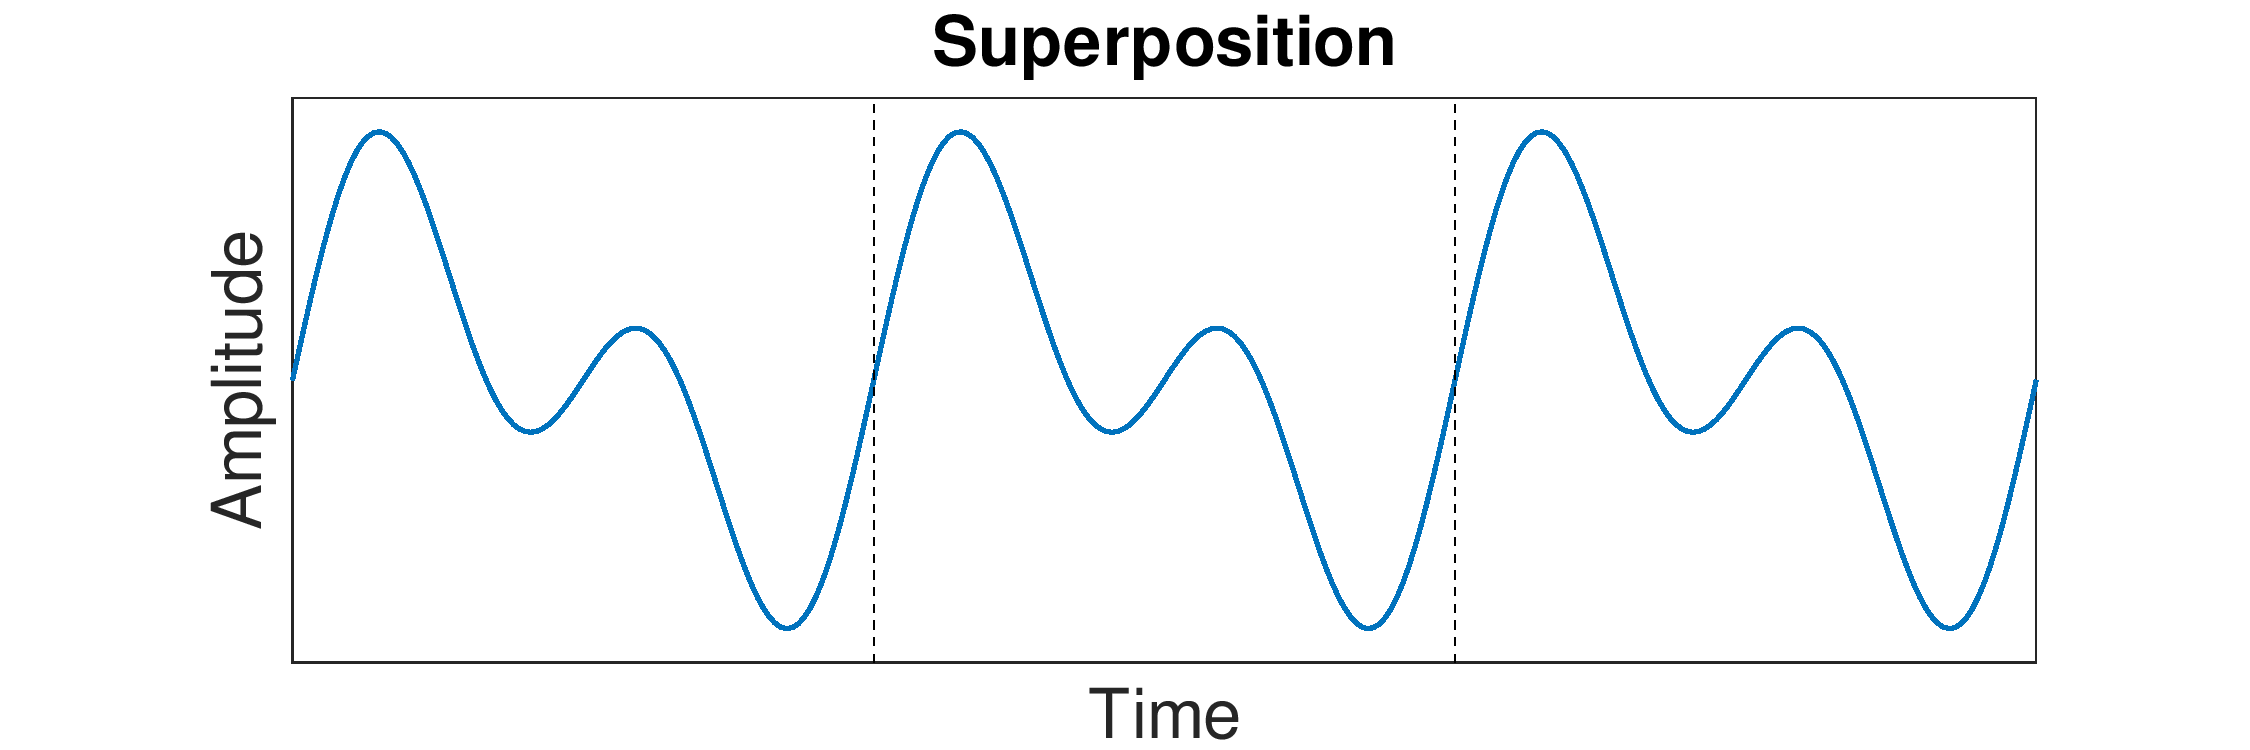
\includegraphics[align=c, width=0.4\textwidth,
		trim={3.5cm 0 3.5cm 0},clip]
		{HarmonyOctaveSuper}\\
\end{tabular}

\centering

{\bf Fifth Interval}
\begin{tabular}{c c c}
	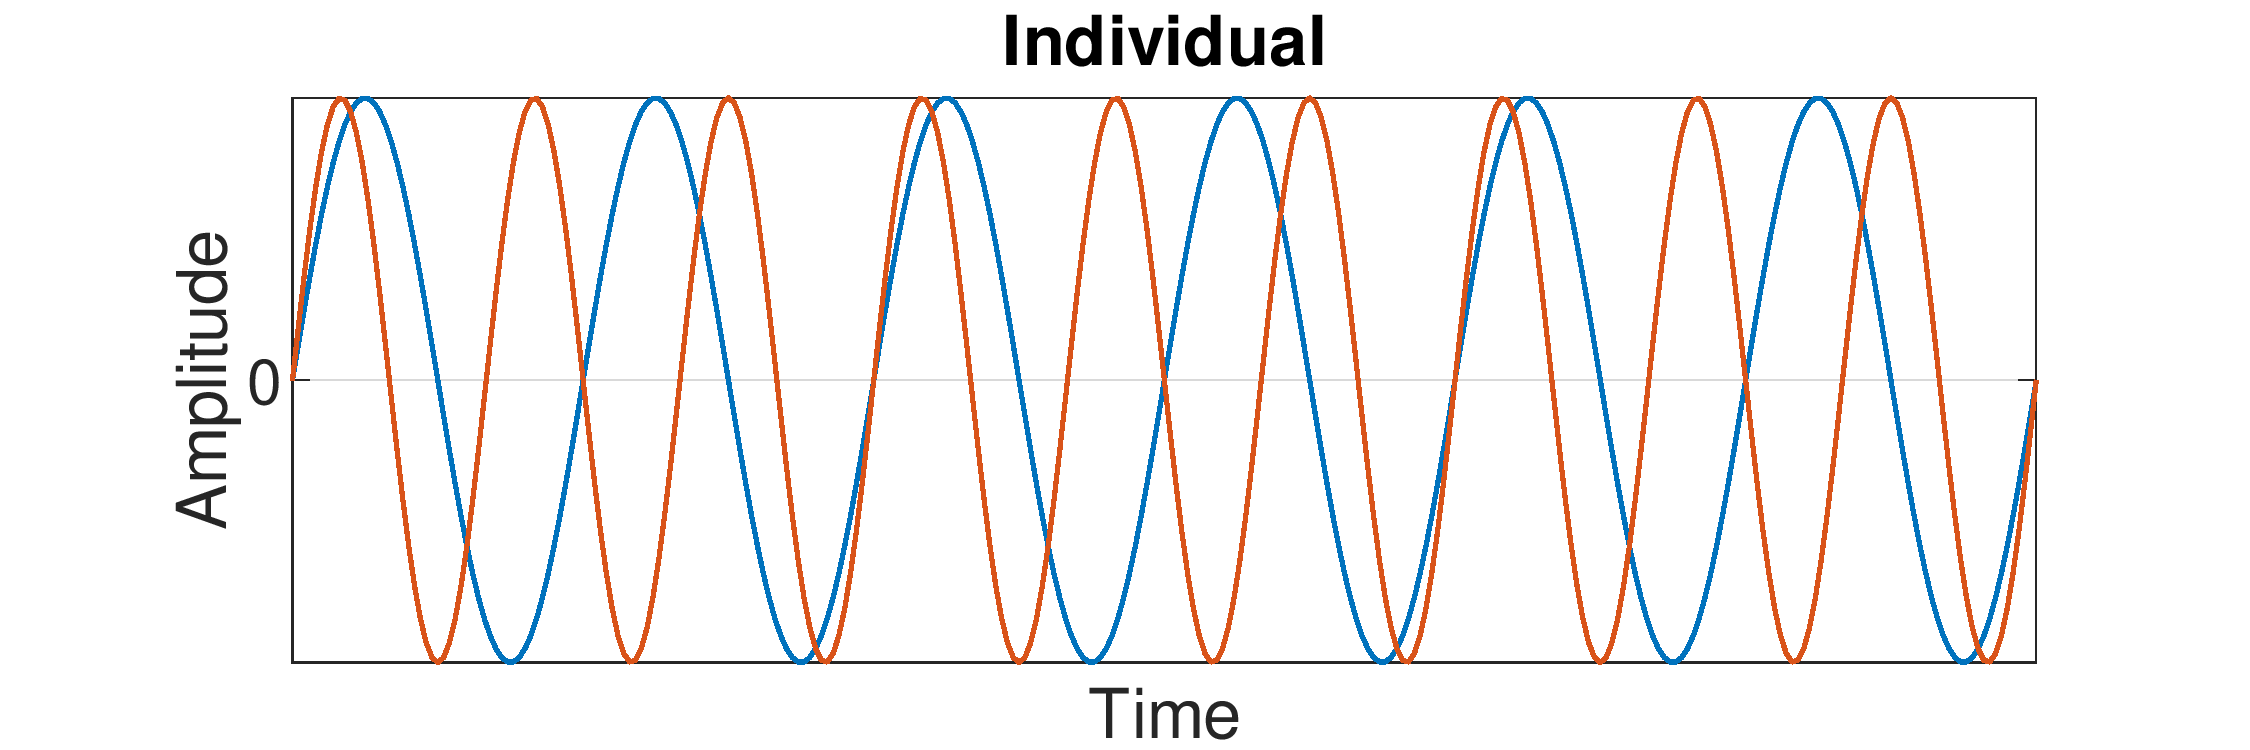
\includegraphics[align=c, width=0.4\textwidth,
		trim={3.5cm 0 3.5cm 0},clip]
		{HarmonyFifthSeparate}
	& \huge$\rightarrow$ &
	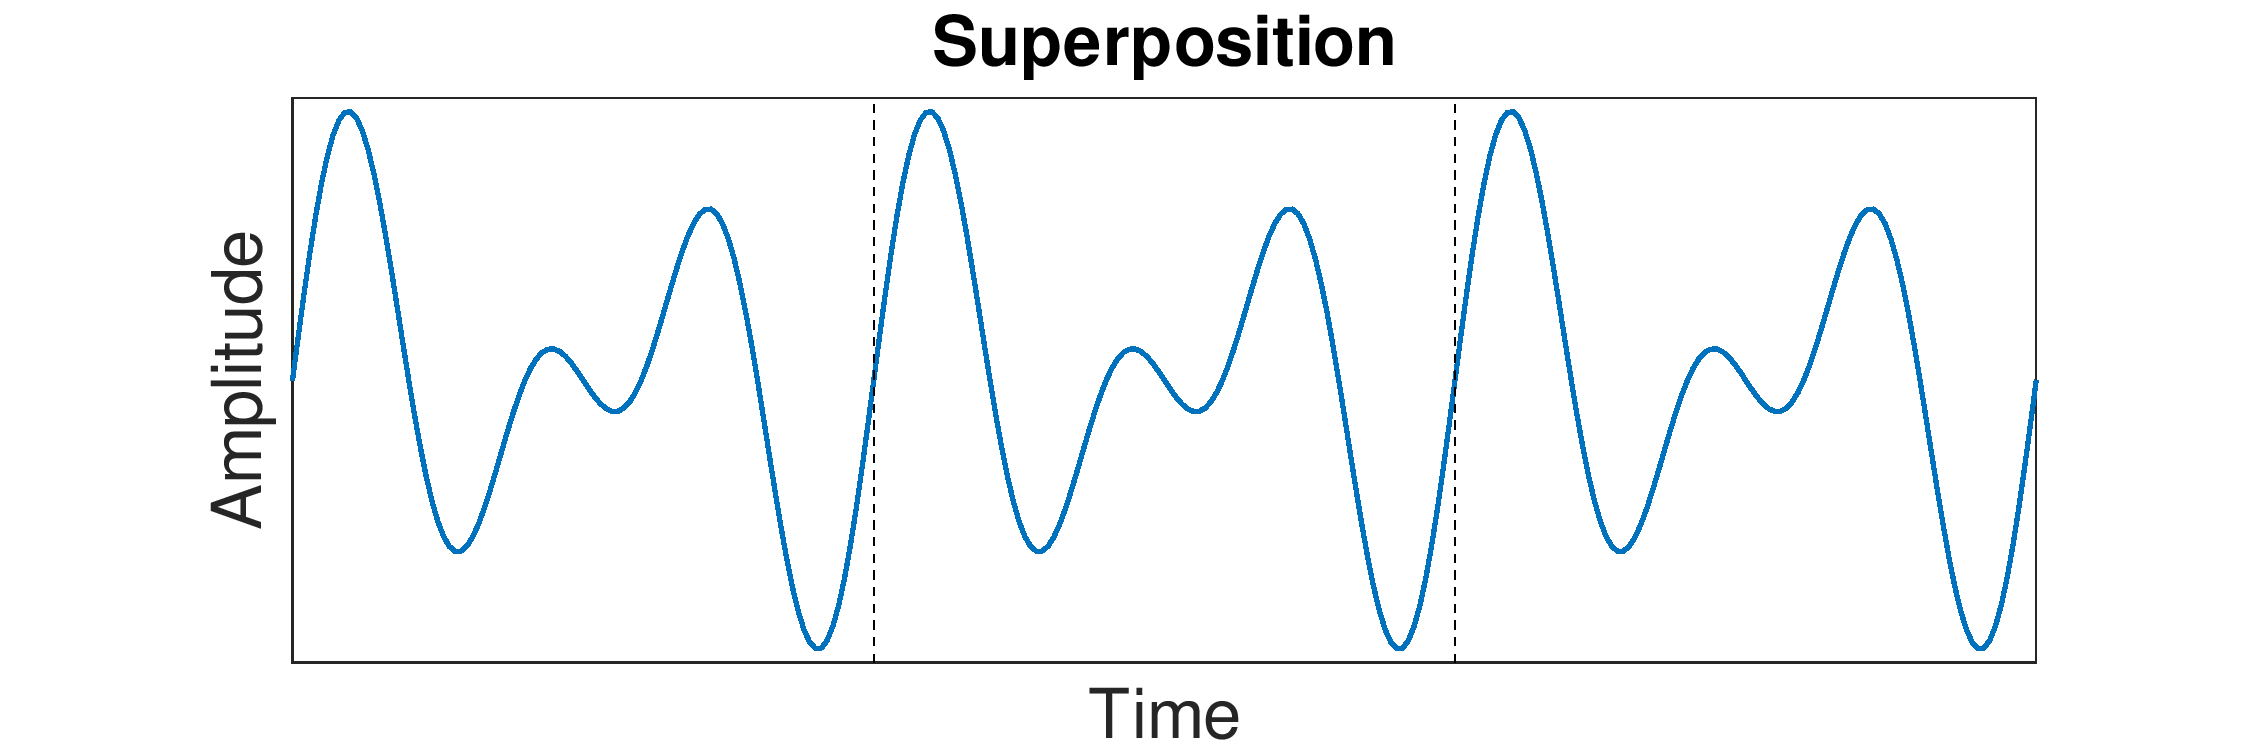
\includegraphics[align=c, width=0.4\textwidth,
		trim={3.5cm 0 3.5cm 0},clip]
		{HarmonyFifthSuper}\\
\end{tabular}
\caption{Harmonic interference of two intervals}
\label{fig:Harmony}
\end{figure}

This concept of harmony gives a simple method to start creating a list of
frequencies that would sound good together. This list is created by starting with
an arbitrary frequency (440 Hz) and using these simple harmonic ratio's to create
a scale. In table \ref{tab:JustTuning} a list of these ratios and corresponding
interval names are given. This is referred to as {\it just tuning}. This tuning
method was naturally discovered because it corresponds to the different modes by
which a string vibrates when plucked\cite{Strings}.

\begin{table}[h]
\centering
\caption{Interval Names and Ratio's of Just Tuning}
\begin{tabu} to \textwidth { | X[l] | X[c] | X[r] | }
	\hline \bf Interval Name & \bf Ratio  & Frequency relative to 440 Hz \\
	\hline Unison & 1/1 = 1.000 & 440 Hz \\
	\hline Minor Second & 16/15 = 1.067 & 469 Hz \\
	\hline Major Second & 9/8 = 1.125 & 495 Hz \\
	\hline Minor Third & 6/5 = 1.200 & 528 Hz \\
	\hline Major Third & 5/4 = 1.250 & 550 Hz \\
	\hline Perfect Fourth & 4/3 = 1.333 & 587 Hz \\
	\hline Tritone & 7/5 = 1.400 & 616 Hz \\
	\hline Perfect Fifth & 3/2 = 1.500 & 660 Hz \\
	\hline Minor Sixth & 8/5 = 1.600 & 704 Hz \\
	\hline Major Sixth & 5/3 = 1.667 & 733 Hz \\
	\hline Minor Seventh & 15/8 = 1.778 & 782 Hz \\
	\hline Major Seventh & 15/8 = 1.875 & 825 Hz \\
	\hline Octave & 2/1 = 2.000 & 880 Hz \\
	\hline
\end{tabu}
\label{tab:JustTuning}
\end{table}

Unfortunately this just tuning method posed a problem when harpsichords and
clavichords (piano-like instruments) were introduced. These instruments required
to be in tune for any starting note. For a tuning system to allow this, a small
interval is required that touches all the wanted intervals when each successive
note is found using this small interval. Since pitch is logarithmically
dependent on frequency, we require a single real number, r, raised to the power of
a subset, n, of positive integers such that the result contains all the desired
interval ratios. Equation \ref{eq:HarmonyRequirement} shows what is required in
unambiguous notation.

\begin{equation}\label{eq:HarmonyRequirement}
	\exists r \in \mathbb{R} \text{ s.t. }
	R \subseteq \{ r^n | n \in \mathbb{N}_0 \}
	\text{ where } R = \{ \frac{1}{1}, \frac{16}{15}, \frac{9}{8}, \frac{6}{5}, \dots \}
\end{equation}

This in not possible and is proved in Appendix A. The best one can do is choose
which interval to keep perfect across all starting notes and choose a sufficiently
small sub-division such that each of the wanted harmonic ratio's is close enough
to an available note such that it is imperceptible to the listener. This is
exactly what equal tempered tuning does. The interval kept constant is the octave
and it is divided into 12 sub-intervals called semitones.  Each semitone interval
is equal to $\sqrt[12]{2}$. This interval has the property of when successively
applied 12 times it produces an octave interval. It also very closely matches all
the required just tuning ratios found in table \ref{tab:JustTuning}.

\begin{table}[h]
\centering
\caption{Interval Names and Ratio's of Equal Tempered Tuning}
\begin{tabu} to \textwidth { | X[l] | X[c] | X[r] | }
	\hline \bf Interval Name & \bf Ratio  & Frequency relative to 440 Hz \\
	\hline Unison & $(\sqrt[12]{2})^0 = 1.000$ & 440 Hz \\
	\hline Minor Second & $(\sqrt[12]{2})^1 = 1.059$ & 466 Hz \\
	\hline Major Second & $(\sqrt[12]{2})^2 = 1.122$ & 494 Hz \\
	\hline Minor Third & $(\sqrt[12]{2})^3 = 1.189$ & 523 Hz \\
	\hline Major Third & $(\sqrt[12]{2})^4 = 1.259$ & 554 Hz \\
	\hline Perfect Fourth & $(\sqrt[12]{2})^5 = 1.334$ & 587 Hz \\
	\hline Tritone & $(\sqrt[12]{2})^6 = 1.414$ & 622 Hz \\
	\hline Perfect Fifth & $(\sqrt[12]{2})^7 = 1.498$ & 659 Hz \\
	\hline Minor Sixth & $(\sqrt[12]{2})^8 = 1.587$ & 598 Hz \\
	\hline Major Sixth & $(\sqrt[12]{2})^9 = 1.681$ & 740 Hz \\
	\hline Minor Seventh & $(\sqrt[12]{2})^{10} = 1.781$ & 784 Hz \\
	\hline Major Seventh & $(\sqrt[12]{2})^{11} = 1.887$ & 831 Hz \\
	\hline Octave & $(\sqrt[12]{2})^{12} = 2.000$ & 880 Hz \\
	\hline
\end{tabu}
\label{tab:EqualTemper}
\end{table}

Table \ref{tab:EqualTemper} shows the modern equal tempered tuning ratios and
their related interval names. For all western scales a subset of these frequencies
are taken to produce the desired scale. Figure \ref{fig:JustVsEqual} shows a
scatter plot of the ratio's of just tuning and equal tempered tuning and a plot of
the percentage error for each note. It can be seen that for each just tuning ratio
needed, an equal tempered tuning note is not far off. The largest error that the
equal tempered tuning scale has, is less than 2\%.  This is considered small
enough to be mostly imperceptible. This twelve tone equal temperament tuning
system is what most modern digital instruments are based on\cite{EqualUsage}.

\begin{figure}[h]
\begin{tabular}{c c}
	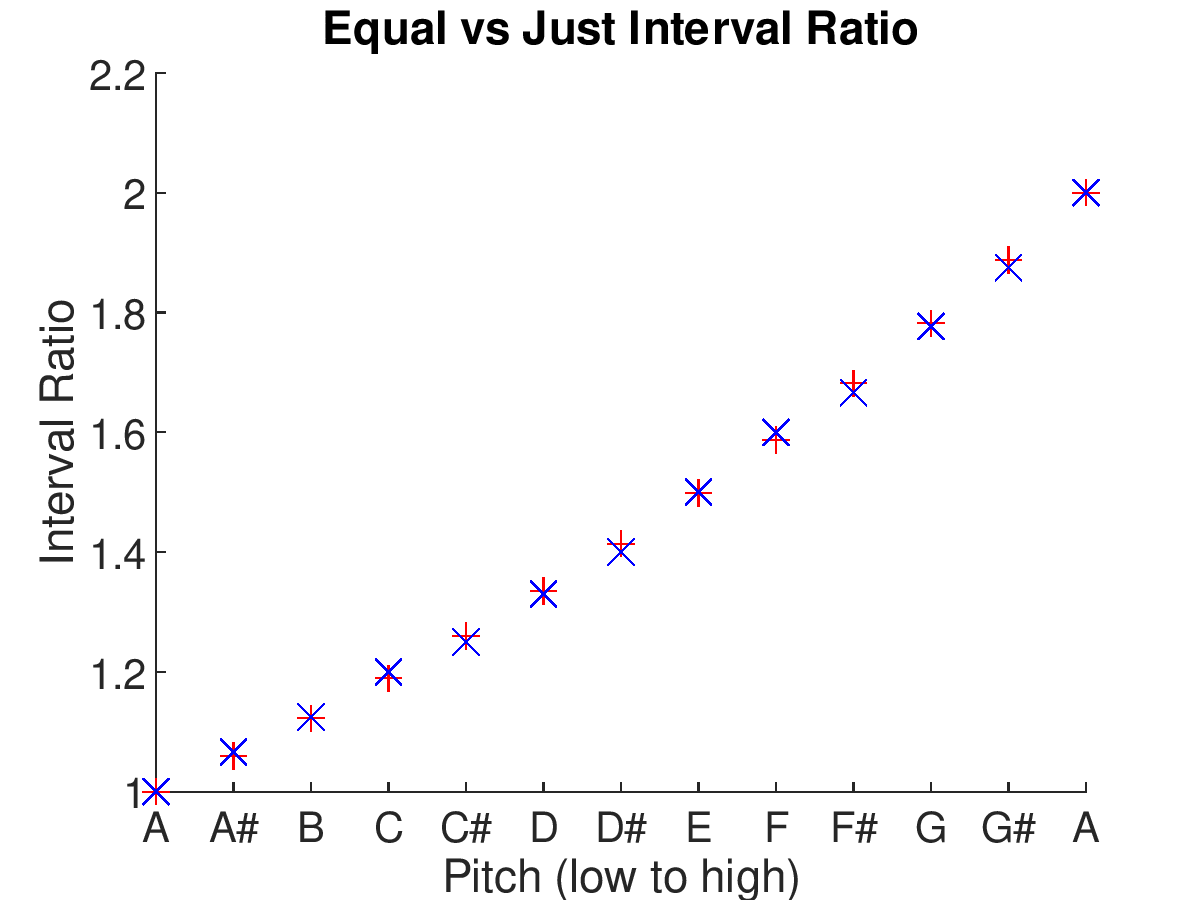
\includegraphics[align=c, width=0.5\textwidth]
		{EqualVsJust}

	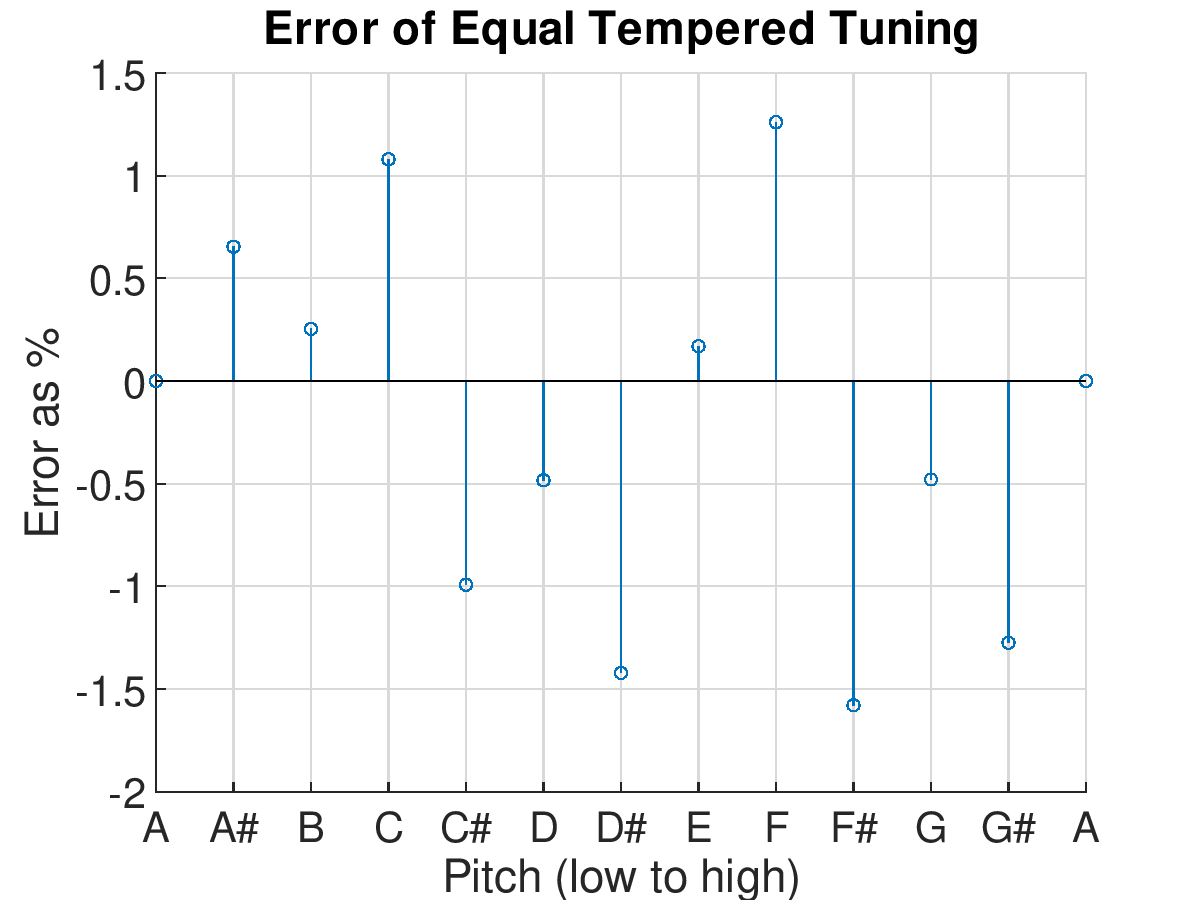
\includegraphics[align=c, width=0.5\textwidth]
		{ErrorEqual}\\
\end{tabular}
\caption{Comparison of just tuning and equal tempered tuning}
\label{fig:JustVsEqual}
\end{figure}

Table \ref{tab:EqualTemper} finally gives us a definition of what is considered to
be correct frequency. Other tuning methods exist but since twelve tone equal
tempered tuning is the most used, it will be considered the objective of this
project. Now that the idea of a correct pitch is well-known, the general pitch
correction structure is investigated.

\section{General Pitch Correction Structure}

As discussed in the ``History of Audio Pitch Correction'' section in the
introduction, there are currently three modern pitch correction systems accessible
for guidance:
AutoTalent\cite{AutoTalent},
AutoTune\cite{AutoTunePatent} and
Smule\cite{SmulePatent}.
The easiest system to get information from is the open source AutoTalent code. The
other two are proprietary and the only reliable information found is that
contained in their patents.

\begin{figure}[h]
	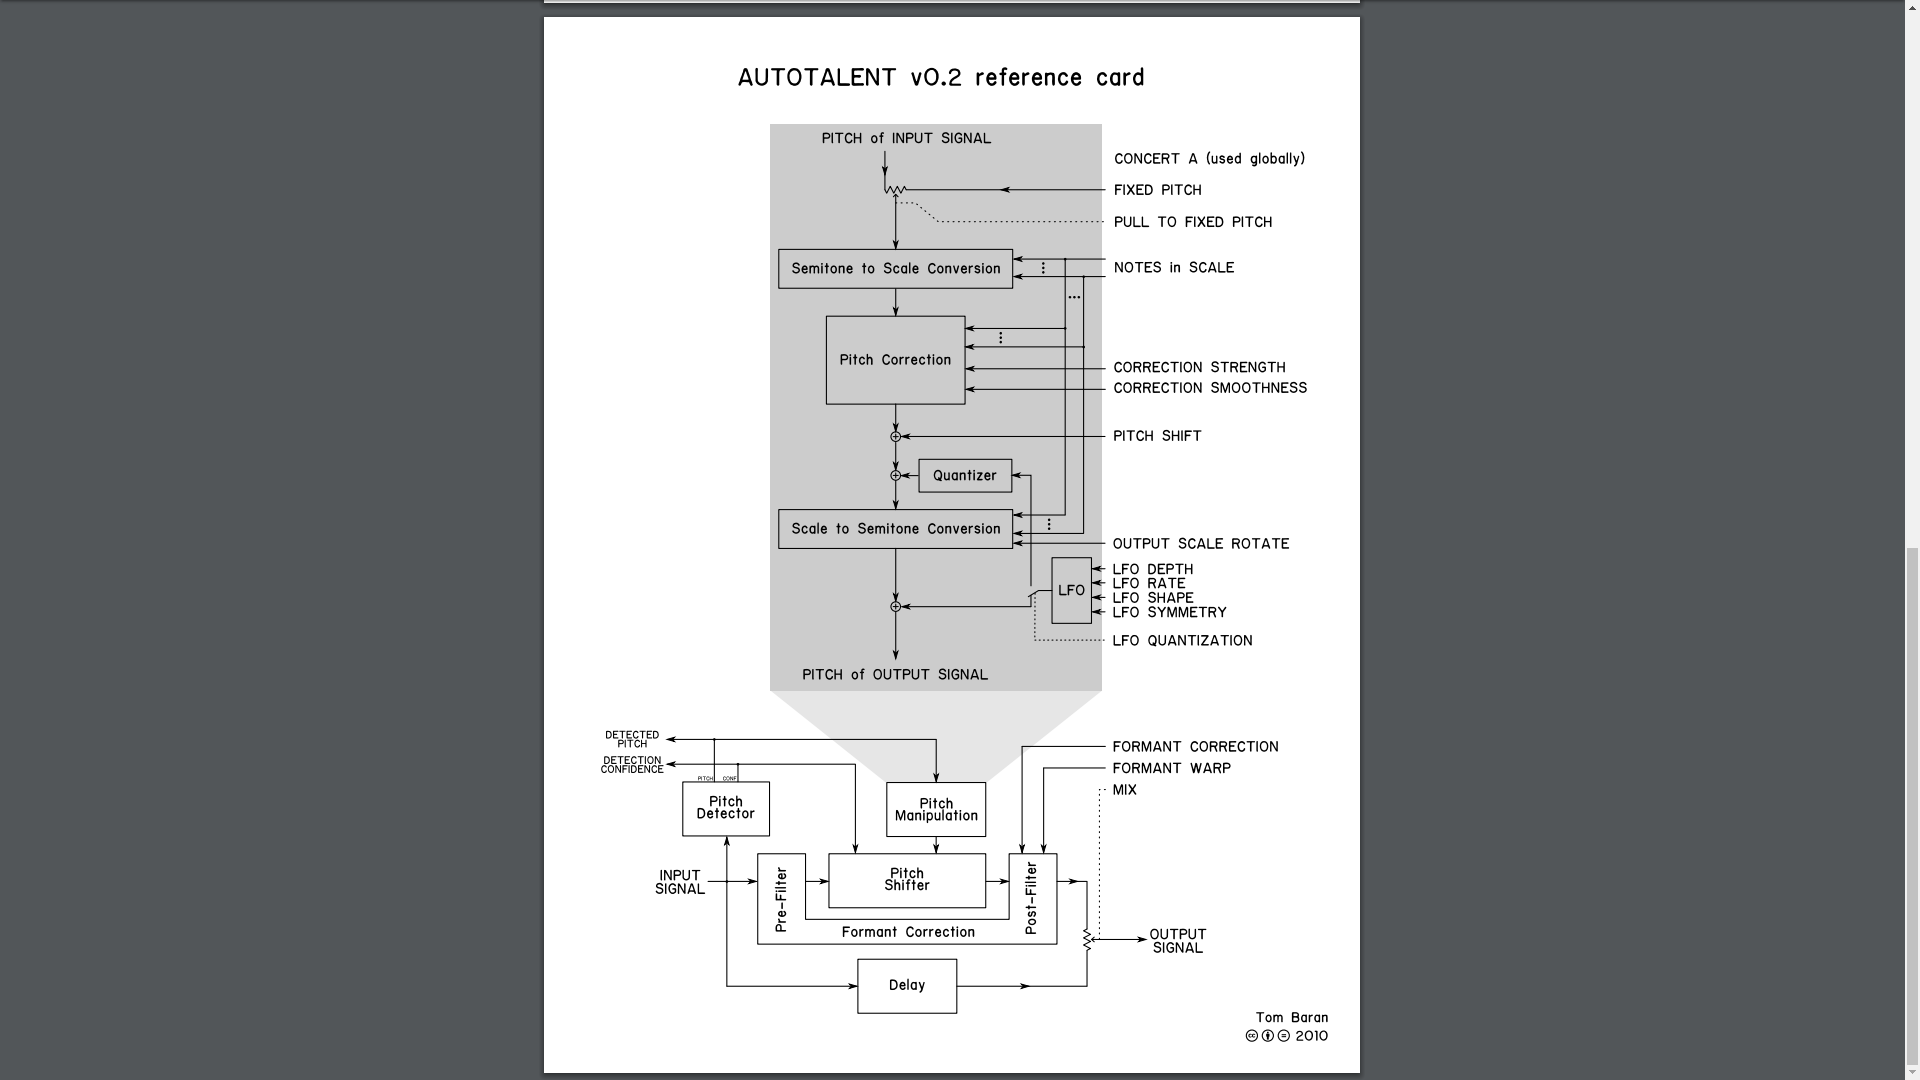
\includegraphics[width=\textwidth, trim={20cm 1cm 20cm 25cm},clip]
	{AutoTalentFlowDiagram}
	\caption{AutoTalent Flow diagram\cite{AutoTalent}}
	\label{fig:AutoTalent}
\end{figure}

On Tom Baran's AutoTalent website\cite{AutoTalent}, there is some explanation of
how his pitch corrector works. Figure \ref{fig:AutoTalent} shows a section of the
flow diagram provided by him for his explanation. The full flow diagram is in
Appendix B. The input signal is supplied to a pitch detector. This detector works
using a type of autocorrelation function mentioned in his explanation on the
website. The detected pitch is passed to a pitch manipulation block which is a
slightly complicated algorithm(see Appendix B) to choose which pitch the pitch
shifter will attempt to shift the output to. A confidence metric is also provided
by the pitch detector and eventually used by the pitch shifter to reduce the
effect when confidence is low. The pitch shifter works using a PSOLA algorithm and
is claimed to produce less artifacts than a phase vocoder based pitch shifter. A
formant correction pre and post filter is also provided.

Formants are the regions in the spectrum where the harmonics of a vocal signal as
a group, peaks\cite{Formants}. The location and size of these formants don't
naturally change, but do when pitch is synthetically shifted. This formant filter
is an attempt at keeping the regions of the formants consistent before and after
the synthetic pitch shift. In the source code for AutoTalent, Tom Baran mentions
that he considers the formant filter experimental\cite{AutoTalent}.

The AutoTune patent\cite{AutoTunePatent} contains some flow diagrams explaining
the workings of the pitch corrector invention. These are very cumbersome and
deemed to be unnecessary, even for an appendix. The basic structure is very
similar to figure \ref{fig:AutoTalent} and figure \ref{fig:SmulePatent}. The
patent suggests the use of a modified autocorrelation function to detect the
pitch and a method by Lent\cite{LentPitchShifter} to shift the pitch.

The Smule patent\cite{SmulePatent} was investigated for hints about what structure
and sub modules were used for their application. From figure \ref{fig:SmulePatent}
it can be seen that they have two streams. A melody stream and a harmony stream.
The harmony stream is irrelevant for pitch correction and will be ignored. The
first block in the melody stream is a low pass filter, downsampler and decimater.
This block represents the analog to digital converter and some pre-processing for
the rest of the system. Thereafter a pitch detection algorithm finds the pitch
being sung. This information, with the pre-processed signal and a target pitch is
fed into a pitch shifting algorithm(PSOLA) to correct the pitch. The target pitch
is found by some pitch choosing algorithm that uses the knowledge of what
harmonies and scale the music is written in.

\begin{figure}[h]
	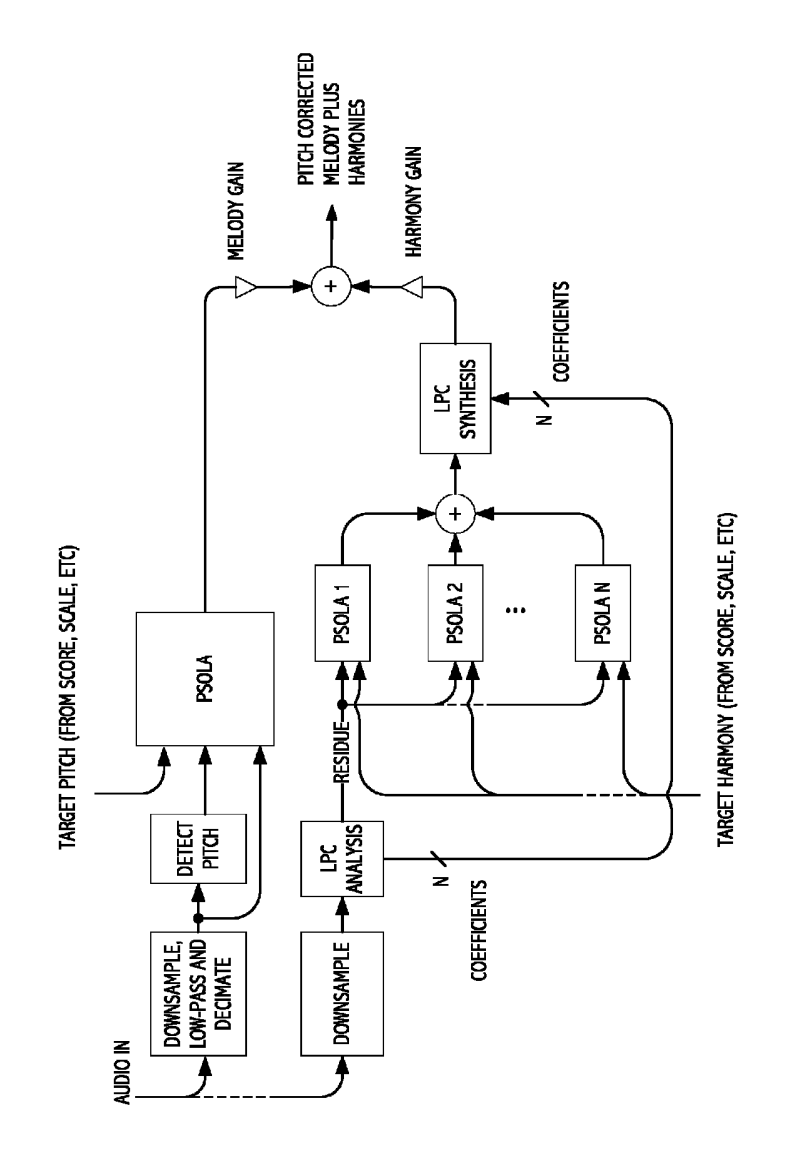
\includegraphics[angle=-90,width=\textwidth, trim={5mm -1cm 5mm 0cm},clip]
	{SmulePatent}
	\caption{Smule patent Flow diagram\cite{SmulePatent}}
	\label{fig:SmulePatent}
\end{figure}

All three pitch correction systems seem to have some common aspects. They are
separated into a frequency detector, a pitch choosing algorithm and a frequency
scaling algorithm. Each system has some additional structures other than the basic
pitch correction added, either to improve the result or for additional features.
The major modules will be investigated further.

\section{Frequency Detection}

Frequency detection is an essential step in the pitch corrector system. Before the
pitch can be corrected, it must be known what the current pitch value is. In the
field of study, the term pitch detection and frequency detection is
interchangeable terms. Both refer to finding the fundamental frequency of a
periodic or semi-periodic signal\cite{ComparitivePitch}. There are several methods
used depending on the application, but all fall under two categories: Time domain
methods and frequency domain methods\cite{PDABook}.

The time domain methods detects the frequency or timing of some time domain
feature that has a known relation to the fundamental frequency of the signal.
Examples of features commonly used are peaks and zero crossings. Some time domain
methods use auto-correlation to measure similarity between a signal and
time-lagged visions of that signal\cite{PDABook}.

Frequency domain methods use operations similar to a Fourier-Transform to inspect
the frequency components of a signal. Windowing the signal is recommended to
reduce spectral smearing\cite{Windowing}.

The methods chosen to be investigated is the zero-crossing method and the
autocorrelation method. These were chosen because of their simplicity and
surprisingly good performance\cite{ComparitivePitch}. Frequency domain methods
were planned to be investigated and implemented but by the end was not time
permitting.

\subsection{Zero Crossing Method}

The zero-crossing method is a time domain method which uses the zero-crossings to
determine the period, and hence, the fundamental frequency of the signal. There
are two zero crossings in a single period, therefore this detector can produce
results at a rate of twice the lowest frequency of the signal. Frequency is
related to period by equation \ref{eq:PeriodVsFreq}.

\begin{equation}\label{eq:PeriodVsFreq}
	F_0 = \frac{1}{p} = \frac{1}{2\Delta s}
\end{equation}

Before the signal is passed to the zero-crossing detector some preprocessing is
done to accentuate some features. Linear predictive coding is a common
preprocessing step used when a zero-crossing detector is used\cite{PDABook}.
Figure \ref{fig:ZeroCrossing} shows a simple graph of how the zero-crossing
detector works. It calculates the time elapsed between two consecutive zero
crossings and uses \ref{eq:PeriodVsFreq} to calculate the fundamental frequency.

\begin{figure}[h]
	\label{fig:ZeroCrossing}
	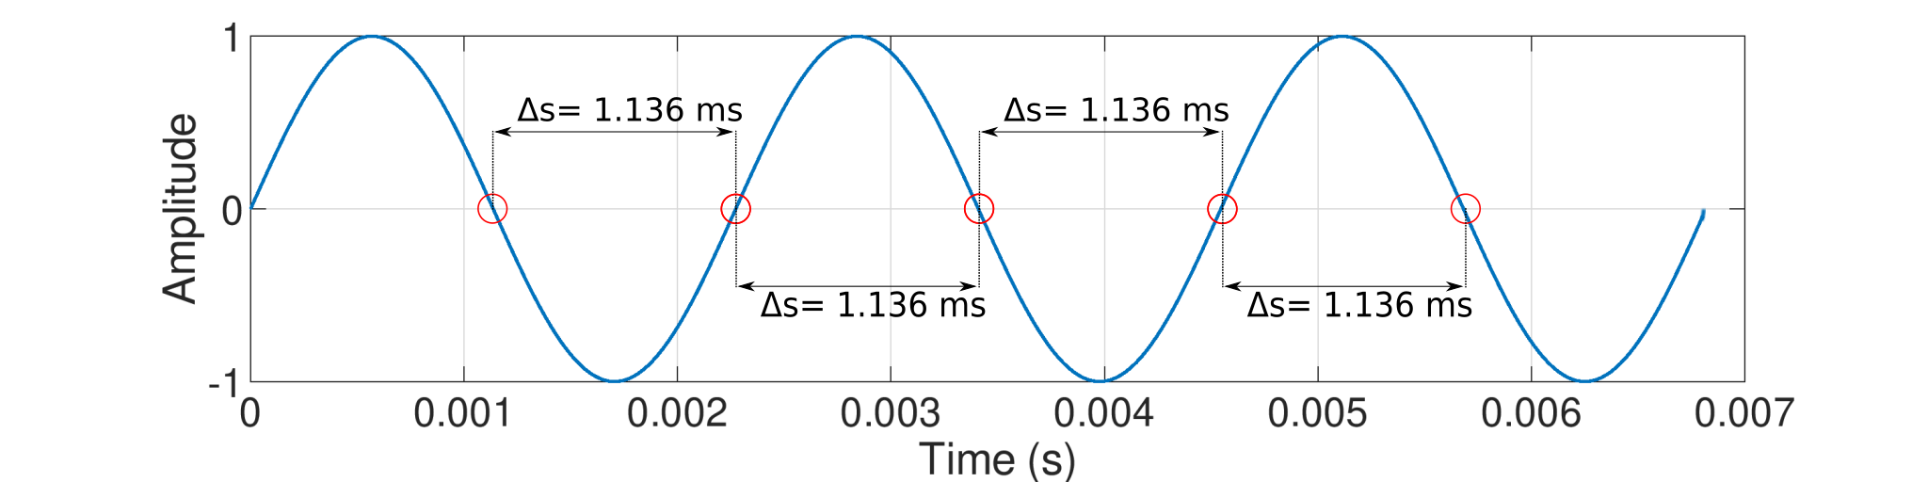
\includegraphics[width=\textwidth]{ZeroCrossingSimple}
	\caption{Zero crossing detector on 440 Hz sinusoidal signal}
\end{figure}

Some obvious implementation details and issues can be conceived but was not found
to be exhaustively investigated in the literature on the subject. Since this is
regarded as a very basic pitch detection algorithm these issues were personally
solved and is further discussed in the implementation section.

\subsection{Autocorrelation Method}

As mentioned previously, the autocorrelation method or variants of it seem to be
popular among prior art. The AutoTune patent\cite{AutoTunePatent} mentions that it
uses a variant of the Algorithm and it appears in the source code and explanations
of AutoTalent\cite{AutoTalent}. Smule mentions autocorrelation, among other pitch
detection methods, in their patent\cite{SmulePatent}.

The original algorithm for pitch extraction using autocorrelation was first
described in a paper written in 1967\cite{OriginalAutocorrelation}. A flow
diagram of the method described in the original paper was produced by a paper
comparing different pitch detection algorithms\cite{ComparitivePitch}. This flow
diagram is shown in figure \ref{fig:AutocorrelationFlowDiagram}. The algorithm in
the flow diagram differs slightly to the algorithm suggested by the original
paper. The original algorithm does not have an infinite peak clipper and
calculates the clipping threshold differently.

\begin{figure}[h]
	\includegraphics[width=\textwidth]{AutocorrelationFlowDiagram}
	\caption{Autocorrelation Algorithm Flow diagram\cite{ComparitivePitch}}
	\label{fig:AutocorrelationFlowDiagram}
\end{figure}

\begin{wrapfigure}{L}{0.35\textwidth}
	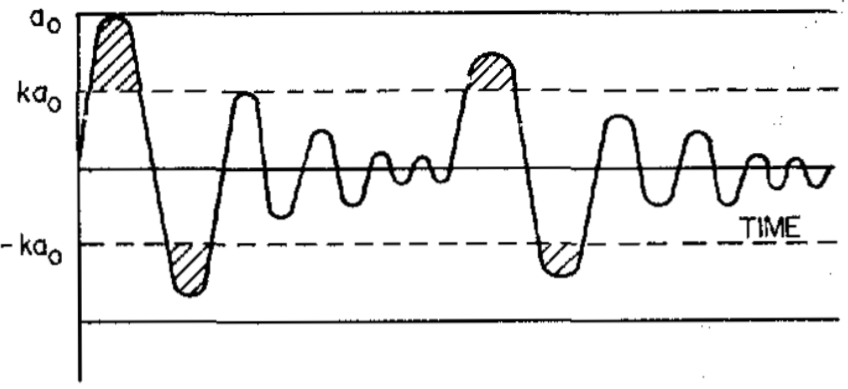
\includegraphics[width=0.35\textwidth]{clip1}
	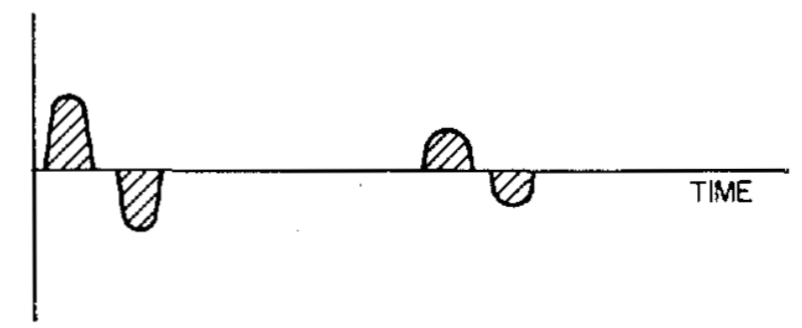
\includegraphics[trim={-13mm, 0mm, 0mm, 0mm},clip,width=0.35\textwidth]
	{clip2}
	\caption{Center Clipping \cite{OriginalAutocorrelation}}
	\label{fig:CenterClipper}
\end{wrapfigure}

The flow diagram algorithm has a pre-processing step that applies a low pass
filter to the signal and breaks the signal up into 30ms overlapping segments.
Next, center clipping is applied to a segment of the signal. The thresholds for
the clipper, $ka_0$, is calculated by first obtaining $IPK_1$ and $IPK_2$, the
maximum of the absolute value of the first and last third of the signal segment
respectively. The threshold is set to k times the minimum value of $IPK_1$ and
$IPK_2$. The value of k is a tuning parameter and a suggested value of 0.67 is
given. A center clipper is then applied to the signal as shown in figure
\ref{fig:CenterClipper}. The autocorrelation of this center clipped signal is then
calculated. The difference in position of the first peak after the center peak is
calculated. The size of this difference is the period of the signal and the peak
of the signal, compared with the main peak, provides a confidence metric.

Center clipping removes information on formants but preserves
periodicity\cite{CenterClippingFormants}. The presence of formants is considered
the cause for inaccurate pitch detection using autocorrelation methods.

\section{Frequency Scaling}

Since pitch is logarithmically dependent on frequency, as shown in figure
\ref{fig:FrequencyVsPitch}, the act of pitch shifting is analogous to frequency
scaling. This is due to one of the logarithmic identities and is shown in equation
\ref{eq:LogLaw}.

\begin{equation}\label{eq:LogLaw}
\begin{split}
	p=\log{(f)} & \text{\hspace{1cm} (given)}\\
	p_{shifted}=p+\Delta p & \text{\hspace{1cm} (pitch shifting)}\\
	\downarrow \hspace{1cm} \\
	\log{(f_{scaled})}=\log{(f)}+\log{(\Delta f)}
	& \text{\hspace{1cm} (substitute)}\\
	f_{scaled}=f\cdot\Delta f
	& \text{\hspace{1cm} (frequency scaling)}
\end{split}
\end{equation}

The general approach taken when doing frequency scaling is to expand or shorten
the signal without affecting the pitch and thereafter re-sampling this expanded or
shortened version to be the same length as the original.

\color{red}
To do:
\begin{itemize}
	\item General approach is to expand/extrapolate frequency
	\item Time domain approaches and frequency domain approaches
	\item Introduce two approaches Phase Vocoder and pitch synchronous overlap and add
\end{itemize}
\color{black}

\subsection{Phase Vocoder}

\color{red}
To do:
\begin{itemize}
	\item Describe method roughly
	\item More in depth description comes in implementation section
\end{itemize}
\color{black}

\subsection{PSOLA}

\color{red}
To do:
\begin{itemize}
	\item Describe method roughly
	\item More in depth description comes in implementation section
\end{itemize}
\color{black}
